\documentclass[12pt]{article}
\usepackage{amsmath,physics,amssymb,array,blindtext,graphicx}
\usepackage[margin=1.5cm,top=1.5cm,bottom=1.5cm]{geometry}
\usepackage{multirow,hyperref,xcolor,listings,comment}

\definecolor{codegreen}{rgb}{0,0.6,0}
\definecolor{codegray}{rgb}{0.5,0.5,0.5}
\definecolor{codepurple}{rgb}{0.58,0,0.82}
\definecolor{backcolour}{rgb}{0.95,0.95,0.92}

\lstdefinestyle{mystyle}{
    backgroundcolor=\color{backcolour},   
    commentstyle=\color{codegreen},
    keywordstyle=\color{magenta},
    numberstyle=\tiny\color{codegray},
    stringstyle=\color{codepurple},
    basicstyle=\ttfamily\footnotesize,
    breakatwhitespace=false,         
    breaklines=true,                 
    captionpos=b,                    
    keepspaces=true,                 
    numbers=left,                    
    numbersep=5pt,                  
    showspaces=false,                
    showstringspaces=false,
    showtabs=false,                  
    tabsize=2
}

\lstset{style=mystyle}

\begin{document}
\title{\textbf{CS3101\\Flight Reservation System}}
\author{G. Sushanth, 19MS134$^*$\\Surendra Bhattarai, 19MS136\footnote{equal contribution}\\Krushna Ranjan Pradhan, 19MS133$^*$\\Rudraksh Agarwal, 19MS080$^*$\\Supratik Sarkar, 19MS137$^*$}
\date{}
\maketitle
\thispagestyle{empty}

\vspace{3cm}
\noindent \textbf{\textsc{\,   INDIAN INSTITUTE OF SCIENCE EDUCATION AND RESEARCH - KOLKATA}}
	\vspace{1.8cm}
  
\begin{figure}[!h]
\centering

\includegraphics[scale=0.45]{ii}
\end{figure}

\pagebreak
%\tableofcontents
\pagenumbering{roman}
\pagebreak
\pagenumbering{arabic}

\section{Task}
Design an interactive flight reservation system in C programming language. The
customer should be able to choose a flight from a calendar through a unique customer id
and see the availability of tickets. Each customer should be given three options for a
ticket: infant, child and adult, with different prices. After the customer chooses the
booking options, the system should generate the final ticket amount.\\

It should have two modes of access (i) Admin and (ii) User. The allowed operations for
each of these modes are:\\
\indent Admin - Make modifications in flight details.

User - Booking.

There should be unique login ids for each. The system should ask for the login id and
check it against a list. The admin and user ids for a person should be different. A person
without a valid id should not be allowed to access the system. An Admin should be one
related to the airport/airlines authorities. Users are the customers.

Each flight should have a unique id, availability, timing, source, destination etc.

In addition, a search facility should be present for both these modes allowing free-text
search in general and also for specific fields of a flight.

\section{Documentation}
\subsection{System Requirements:}
This code can be compiled using Visual Studio Code or Dev C++. This code is written on Windows 8/10 operating systems.

\subsection{Header Files and standard functions}
%<windows.h>
%Structures and Functions

%COORD = {x,y} - Defines the coordinates of a character cell in a console screen buffer
%SetConsoleCursorPosition() - Function for setting the console in the required position.

\noindent \textbf{\texttt{<stdio.h>}}
\begin{itemize}
\item \texttt{printf()} - This function is used to print float, integer, character, string, octal and hexadecimal values on screen.

\item \texttt{scanf()} - This function reads a character, string, numeric data from user and store it in a variable.

\item \texttt{fprintf()} - This prints content in file instead of stdout console.

\item \texttt{fscanf()} - This reads set of characters from file and returns EOF at the end of the file.

\item \texttt{fopen()} - This function opens a file to perform operations like reading, writing etc. If a file exists, then that file is opened otherwise a new file will be made.

\item \texttt{fclose()} - This function closes an opened file.

%\item \texttt{putch()} - This function writes a character to file

\item \texttt{fseek()} - This moves file pointer position to a specific location
%SEEK\_CUR - Moves file pointer position to given location
%SEEK_END - Moves file pointer position to the end of file

\item \texttt{fflush()} - This function flushes a file.  Its purpose is to clear (or flush) the output buffer and move the buffered data to console or disk.

\item \texttt{fread()} - This reads \texttt{nmemb} elements (each element is the number of bytes indicated by size) from the stream pointed to by stream and stores them in \texttt{ptr}.

\item \texttt{remove()} - This function removes/deletes a file.

%\item \texttt{ftell()} - This function gives current position of file pointer

%\item \texttt{rewind()} - Moves file pointer position to the beginning of the file

\end{itemize}

\noindent \textbf{\texttt{<time.h>}}\\

It is a header file that contains time and date function declarations to provide standardized access to time and date formatting.\\

\noindent \textbf{\texttt{<conio.h>}}

\begin{itemize}
\item \texttt{getch()} - It reads characters from keyboard
%\item getche() - It reads character from keyboard and displays the outpu on the output screen
\end{itemize}

\noindent \textbf{\texttt{<stdlib.h>}}

\begin{itemize}
\item \texttt{exit(0)} - For exiting the program and closing the application.
\end{itemize}

\noindent \textbf{\texttt{<string.h>}}

\begin{itemize}

\item \texttt{strcmp(str1, str2)} - This compares two strings. It returns 0 if \texttt{str1} is same as \texttt{str2}, returns a number $<$ 0 if \texttt{strl} $<$ \texttt{str2} and a number $>$ 0 if \texttt{str1} $>$ \texttt{str2}.
\end{itemize}

\section{How to execute the program}
When the program is executed, the user will be directed to the main interface. There, the user is to choose usertype (admin or user).

\begin{figure}[!h]
\centering
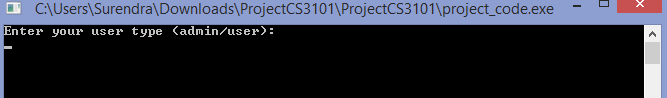
\includegraphics[scale=0.8]{ask for user}
\end{figure}

%%% ADMIN INTERFACE
$\bullet$ \underline{\textbf{If selected \texttt{admin}}}:\\

If selected \texttt{admin}, the admin has to provide his/her username (e.g. indigo) and password (ind123go). Then a welcome note will appear, and the admin is expected to press \texttt{enter}.

\begin{figure}[!h]
\centering
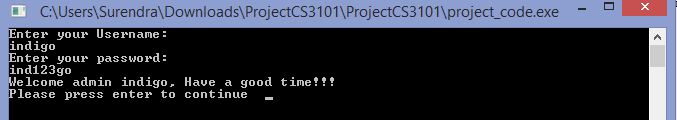
\includegraphics[scale=0.8]{ask for username}
\end{figure} 

Then, the admin is asked what he/she wants to do (Add flight, modify flight or remove flight).

\begin{figure}[!h]
\centering
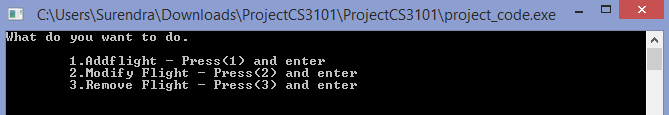
\includegraphics[scale=0.8]{what to do}
\end{figure} 

Choosing option 1 will allow the admin to add flights. In this option, he has to provide the date, timing of flight, names of cities where the flight will depart from and arrive, and provide the expected timing to reach destination. The user has to also enter the unique ID of the flight, which is basically the flight number of the plane. The admin can also add the prices of various tickets in this option.

\begin{figure}[!h]
\centering
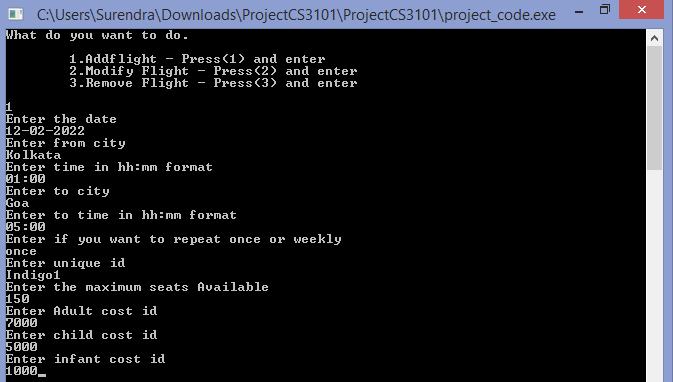
\includegraphics[scale=0.75]{addflight}
\end{figure} 
\pagebreak

Now, the admin can modify some information(s) of flight(s) if he/she wishes by clicking the option 2. \texttt{Modify Flight}. Here, the admin can change departure time, arrival time, costs for adults, children and infants.

\begin{figure}[!h]
\centering
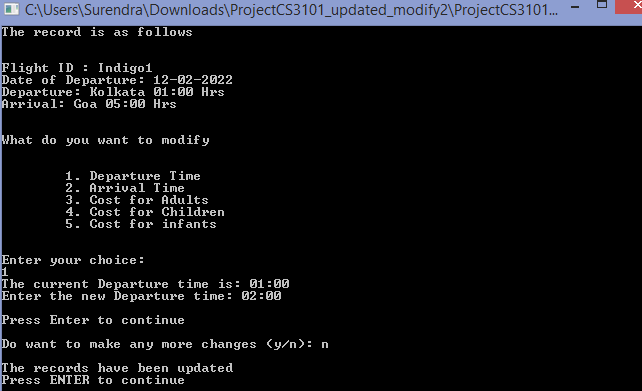
\includegraphics[scale=0.75]{modify1}
\end{figure} 

The admin can also remove any flight by clicking on the option 3. \texttt{Remove Fight}.

\begin{figure}[!h]
\centering
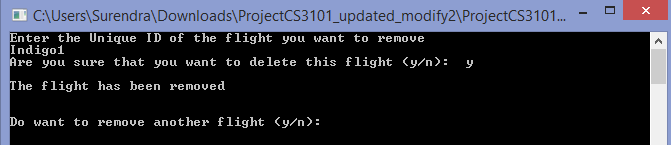
\includegraphics[scale=0.75]{remove}
\end{figure} 

%%%%%%%%%%%%%%%%%%%%%%%%%%%%%%%%%%
%%%%%   USER INTERFACE
%%%%%%%%%%%%%%%%%%%%%%%%%%%%%%%%%

$\bullet$ \underline{\textbf{If selected \texttt{user}}}:\\

If in the main interface, one selects \texttt{user}, four options (reserve, cancel, display or exit the program) will appear which the user can choose from.

The user is asked to provide a date when he/she will travel, and also the place from he/she would like to depart from. Also they need to provide the place where they would like to land.

After that, all available seats will shown. 



\begin{lstlisting}[language=C]
#include<stdio.h>
#include<stdlib.h>
#include<string.h>
#include<time.h>

char Username[20];
char Type[20];
int login(int zeon);
int addflight(char admin[20]);

struct details
    {
        char tname[20]; // Type of user
        char uname[20]; // User name
        char pname[20]; // password
    };


struct flight
    {
        char adateadd[10];
        char aprovider[20];
        char afrom[20];
        char afromtime[5];
        char ato[20];
        char atotime[5];
        char aduration[5];
        char arepeat[10];
        char id[10];
        int adultcost;
        int childcost;
        int infantcost;
        int deleted;
    };
\end{lstlisting}


\section{Contributors}
$\bullet$ G. Sushanth: Admin + user interface, designing control flow of the system, ensuring successful compilation\\

\noindent $\bullet$ Surendra Bhattarai: User interface, documentation, debugging, designing control flow of the system, ensuring successful compilation\\

\noindent $\bullet$ Krushna Ranjan Pradhan: Worked on notifications and warnings, designing control flow of the system\\

\noindent $\bullet$ Supratik Sarkar: Documentation, designing control flow of the system\\

\noindent $\bullet$ Rudraksh Agarwal: Flight adding, designing control flow of the system

\section{Acknowledgement}
We would like to thank our instructor Prof. Kripabandhu Ghosh for giving us such a nice project, where we got to know about so many new functions and modules. This project helped us tremendously because we got know how to use C language to tackle a real life problem.

\end{document}